%\section{Exploratory analysis of team shape in Australian Rules Football using GPS tracking data}
\pagebreak % TODO: Remove page break and fix any layout issues

\section{Exploratory Analysis of Team Shape in \afl{} using GPS Tracking Data}
\label{sec:shapepaper}

This section of the thesis will demonstrate how team GPS tracking can provide value beyond existing datasets that focus on just the ball. % value / insights ?

In preliminary talks with an elite \afl{} club, they expressed interest in team formations and how these change in attack and defence. They hypothesised that the team should contract in defence and spread out in attack, although did not have quantitative evidence of this.

The previous chapters have been building up the foundations for a sport analysis platform. This section builds upon this platform to perform a study of how team formations spread and contract during attack and defence phases of play in \afl{}.

% This is linked with scoring data in order to provide insight into the differences between successful and unsuccessful
%team behaviours.

% \subsection{Abstract}
\subsection{Introduction}

While individual player tracking data can be readily digested by sport practitioners, the high-dimensional nature of whole-team tracking data presents challenges for those seeking to utilise tracking data for team-level strategy analysis. This section of the thesis %paper
introduces a technique for analysing team formations based on how spread out the team is. The approach proves promising as a framework to empower sport practitioners to derive strategic insights from team level GPS tracking data.

% only makes sense as abstract
% Instances where an \afl{} team remained spread out in attack rather than condensing into a pack were associated with fast game speed in which the ball was moved toward goal quickly. The approach proves promising as a framework to empower sport practitioners to derive strategic insights from team level GPS tracking data.

% \subsection{Introduction}
%
% TODO: Introduce AFL, gps tracking devices, need for dimensionality reduction / feature extraction, need for new spatio-temporal analysis techniques to unravel team-level GPS data into a form that sport practitioners can interpret and build upon.

\subsection{Related Work}

This section will briefly highlight existing metrics proposed in the literature for measuring team shape. Early papers focus on analysis of team shape in \soccer{} using player trajectories derived from video \cite{Yue2008, Clemente2013a, Clemente2013b, Folgado2014, Couceiro2014} or local position measurement systems \cite{Frencken2008, Frencken2011}.
Basketball has also been studied \cite{Bourbousson2010b}. Later studies have applied these techniques using GPS systems \cite{Macas2012, Frias2014, Silva2016}. Existing metrics proposed in the literature for measuring team shape include stretch index, surface area, length-to-width ratio, and spatial variability.\footnote{An overview of these metrics is provided in \appendixsecref{appendixsec:measures-of-team-shape}} Alexander et al. (2019) were first to apply these kinds of metrics to AFL \cite{Alexander2019a}, although so far have only studied a simulated drill \cite{Alexander2019a} and later a single \afl{} match \cite{Alexander2019b} using existing approaches designed for \soccer{} and basketball.

Alexander et al.'s initial study \cite{Alexander2019a} examined team length, width and surface area in a 15-v-15 Australian Rules Football simulation match. Team length, width, and surface area were found to be greater when teams were in offence than defence. Alexander et al. noted some counter-intuitive results arising from their methodology, such as teams being centred further back in offence than in defence, which was speculated to be an artefact of the location teams gained possession of the ball.

% Alexander2019a (2018/2019) Summary:
% Summary: "Length, width, and surface area were typically greater during the offensive phase comparative to defensive and contested phases"
% "Length was greater during offence compared to defence for both teams. Although, length during the contested phase was greater than offensive and defensive phases for both teams."
% "Width was greater during offence compared to defence for both teams. Although Team B’s width during contest was smaller during defence compared to the contested phase."
% "Surface area was greater for both teams when comparing offence to defensive and contested phases of play and comparing defence to the contested phase."
% "This is the first study to describe collective team behaviour in AF teams during different phases of match play"

A follow up study by Alexander et al. \cite{Alexander2019b} examined a single competitive AFL match played by the team (however did not have data for the opposition). In alignment with their first study of a 15-v-15 simulation match \cite{Alexander2019a}, the follow up study also found that team length, width, and surface are were greater in offence than defence. They used heat-maps to visualise the typical locations occupied on the field broken down by possession state and which zone of the field the ball was in. They quantified the level of spatial variability in the heat-maps using Shannon Entropy, which revealed lower variability when the ball was contested; however, similar values in offence and defence.

Research is needed to explore whether Alexander et al.'s findings hold for other \afl{} teams over multiple matches, and to test alternative measures of team spread.
% to remove statistical artefacts arising from the location of first possession,


 % which varied by possession  the Shannon Entropy in offence was similar to that when in defence.

 % They used heat-maps to visualise the typical locations occupied on the field. Heat-maps were produced for each combination of possession state (offence, defence, or contest when neither team had clear possession) and quarter of the field (ball in defensive 50 metres, ball in defensive mid-field, ball in forward mid-field, or ball in forward 50 metres). They used Shannon Entropy to quantify the level of spatial variability and found that the Shannon Entropy in offence was similar to that when in defence.

%, specifically the uncertainty as to which point on the field would be occupied by an (unknown) player (i.e. without consideration of player roles)

% (as adapted to sport by Couceiro et al. 2014 \cite{Couceiro2014})

% Alexander2019b Summary:
% "Length was greater during offence compared to defence (4.7; 95% CI 4.2–5.3)"
% "Width was greater during offence when compared to defence (3.3; 95% CI 2.9–3.8)"
% Surface area was greater during offence compared defence (397.5; 95% CI 359.8–435.2) and contest (794.2; 95%).
% (which is strange, as the team won, so would have (possibly) spent more of its time in the smaller F50 zone)
% dispersion as measured by Shannon Entropy is called "variability" by Alexander et al.
% "ShannEn values (Figure 5) were greater during offence and defence compared to contest."
% (examining the figures, the level of Shannon Entropy between offence and defence seems comparable. I'm sceptical about the finding that it was lower in contest -- the plots seem to show that only a few key contest locations appear in the occupancy map, so the lower variability is likely due to only considering a small number of contests)

% "Research into collective team behaviour in Australian Football (AF) also remains largely absent, with only one study reported to date (Alexander et al., 2018)"
% "This is the first study to investigate the influence of match phase and field position on collective team behaviour in AF."

% Vice Sports 2016, "When Is a Point in AFL Worth More Than a Goal? Unpacking the Expected Score Statistic". https://www.youtube.com/watch?v=DXDt00C1spo "distance, angle, pressure on the shooter."

\subsection{Method}

\subsubsection{Datasets}

Three datasets were synchronised and integrated to support the analysis: player position tracking data, possession chain data, and ball position data at time of possessions.

Player position tracking data collected by wearable GPS tracking devices (GPSports) worn by an elite \afl{} club were obtained for matches played during the 2015 season. After removing rounds in which one or more player devices were not working or experienced signal loss, six matches were available, five of which were played at the team's home ground. For consistency only the five home ground matches were selected for analysis.\footnote{See \secref{sec:integration-data-selection-process} for details of the data selection process, and \textit{Experiment Design} below for the rationale for focusing on the home games in this analysis.}

Possession chain data for each match were recorded by the official \afl{} statistics provider Champion Data. A possession chain is a sequence of possessions and disposals (e.g. kicks, handballs) by a single team from the moment of initial ball possession through to a scoring event (e.g. a goal) or loss of possession through a turnover to the opposition or stoppage (e.g. ball out of bounds).

There is no GPS tracking device in the ball; however, Champion Data graphically pinpoint the approximate ball location on a diagram of the field at the time of each possession. The time of these events is reported to be accurate to 5 seconds, and ball position is reported to be accurate to approximately 5 to 10 metres \cite{oshaughnessy_possession_2006}.

\subsubsection{Data Processing}

Team GPS data were anonymised by converting them to a point cloud sequence. This was performed according to the methodology established by Simmons et al. 2018 \cite{Simmons2018} (\secref{sec:Simmons2018}) to ensure the research team did not have access to the underlying player tracking data in (re-)identifiable form at any stage of the project. GPS data were reprojected relative to the local coordinate system of the playing field using the \textit{GPS to XYT} tool designed by Simmons et al. 2017 \cite{Simmons2017} (\secref{sec:Simmons2017}). As the study involved only non-identifiable data, it was granted ethics exemption by Deakin University Human Research Ethics Committee (2018-121: GPS analysis of team shape and game style in elite Australian Rules Football).

The component of the ball position vector in the direction of the goals was used as a proxy measure of how close the team is to scoring a goal. More refined approaches are possible, such as the Euclidean distance from goal, or the \textit{apparent width} \cite{Jackson2016} of goals (in order to account for the apparent narrowing of the goal area when attempting to kick a goal from an angle).

\subsubsection{Team Spread}

The high-dimensional nature of the GPS formations makes analysis difficult in their raw form. The team has 18 players on the field, each with an x,~y dimension (ignoring analysis of jumps), resulting in 36 continuous dimensions, i.e. formations exist in $\mathbb{R}^{36}$. Thus a team spread feature was generated to reduce this to a single dimension, which facilitates visual exploration by humans, as well as reducing risk of over-fitting during analysis. Let team spread at a given time instant be defined as the Root Mean Square (RMS) of player distances from the centroid of the team formation (Eq.~\ref{eq:spread}):

\begin{equation} \label{eq:spread}
spread=\sqrt{\frac{1}{N} \sum_{i=1}^{N} \left((x_i - \bar{x})^2 + (y_i - \bar{y})^2\right)}
\end{equation}

% https://tex.stackexchange.com/questions/36500/how-to-provide-a-definition-for-symbols-in-a-latex-math-equation
\begin{minipage}{\textwidth}
where
\begin{description}
\item[$x_i$] is the x-coordinate of player $i$ at the time instant
\item[$y_i$] is the y-coordinate of player $i$ at the time instant
\item[$\bar{x}, \bar{y}$] are the coordinates of the centroid of the team
\item[$N=18$] is the number of team players on the field
\end{description}
\end{minipage}

This can be thought of as a two-dimensional form of the formula for standard deviation. Loosely, it measures the average distance of players from the centre of the formation (with greater weight being given to players who are further away). In this sense it is similar to the definition of the ``stretch index'' \cite{Yue2008, Bourbousson2010b} used in the literature; however, it uses the quadratic mean (RMS) rather than the arithmetic mean. Prior to the spread calculations, players in the interchange area were removed, which was achieved by removing the four player locations reported as closest to the interchange side of the field. A visual explanation of the spread metric and ball position is shown in \figref{fig:spread-metric-concept}.
%containing the interchange area. % (i.e. furthest to the left-hand side of the field visualisation).

\begin{figure}[!htb]
\centering
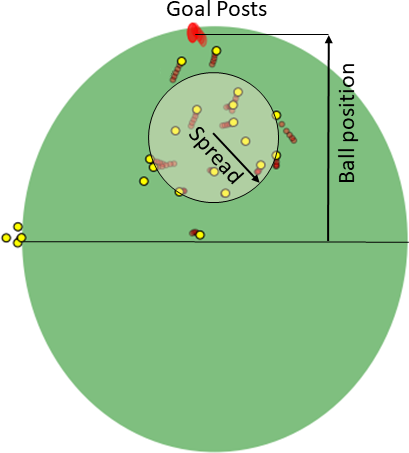
\includegraphics[width=0.5\linewidth]{figs/paper/gps_presentation_spread-metric.png}
\caption{The ball position component in the direction of the attacking goal is used as an indicator of how close the team is to scoring. The team spread feature measures how dispersed the team is relative to the centre of the pack. Interchange players are removed from the spread calculation. See Eq.~\ref{eq:spread} for details.}
\label{fig:spread-metric-concept}
\end{figure}
%\textbf{TODO:} Replace high-level concept slide shown (Powerpoint) with visualisation output overlaid with exact spread value
% Good enough, visual is clear and roughly accurate.

\subsubsection{Experiment Design}
\label{sec:shapepaper-experiment-design}

Alexander et al. \cite{Alexander2019a} noted counter-intuitive results arising as an artefact of the location teams gained possession of the ball. If all possessions are analysed, then the analysis of team shape will be confounded by the influence of the location that the team gains initial possession of the ball. For example, if the team were good at gaining possession of the ball from the opposition near the edge of the field, then the team shape during the attack phase would disproportionately represent the shape of the team near the edge of the field rather than strategic differences between defence and attack formations.

% If data from two teams were available, then the location that one team gains possession and begins attack will correspond to the location that the opposition team begins defence. However, when utilising data from just a single team, ...

To control for these confounding effects, this study compares possession chains in attack and defence from known starting locations. The \centrebounce{} (when an umpire bounces up the ball to begin play) is an example of this, as it always occurs in the centre of the field. Ruckmen are responsible for attempting to hit the ball from the \centrebounce{} to their own team; however, an investigation by O'Shaughnessy noted that the team that gains possession from the \centrebounce{} is ``essentially a coin flip'' \cite{oshaughnessy_identification_2016}. Therefore, the \centrebounce{} can be considered as a form of randomised assignment that can be used to measure the effect of gaining possession. This study will also analyse possession chains beginning with a kick-in, which are always taken from the end of the field.

Limiting the study to only certain possession chains limits the data; however, also strengthens the rigour of the analysis by ensuring that confounding effects are prevented through use of a consistent initial possession location. The utilisation of all five available home matches was essential to ensure sufficient data. While data for a sixth match was available, the field shape for this match differed to the home ground, thus was discarded to ensure a consistent field shape across all samples.

% Alexander2019a (2018/2019) Summary:
% Summary: "Length, width, and surface area were typically greater during the offensive phase comparative to defensive and contested phases"
% "Length was greater during offence compared to defence for both teams. Although, length during the contested phase was greater than offensive and defensive phases for both teams."
% "Width was greater during offence compared to defence for both teams. Although Team B’s width during contest was smaller during defence compared to the contested phase."
% "Surface area was greater for both teams when comparing offence to defensive and contested phases of play and comparing defence to the contested phase."
% "This is the first study to describe collective team behaviour in AF teams during different phases of match play"
% A follow up study by Alexander et al. \cite{Alexander2019b} examined a single competitive AFL match played by the team (however did not include data for the opposition). This study also found that team length, width, and surface are were greater in offence than defence. They used heat-maps to visualise the typical locations occupied on the field. Heat-maps were produced for each combination of possession state (offence, defence, or contest when neither team had clear possession) and quarter of the field (ball in defensive 50 metres, ball in defensive mid-field, ball in forward mid-field, or ball in forward 50 metres). Shannon Entropy was used to quantify the level of spatial variability. The Shannon Entropy in offence was similar to that when in defence.


\subsection{Exploratory Analysis}

\begin{figure}[!htb]
\centering
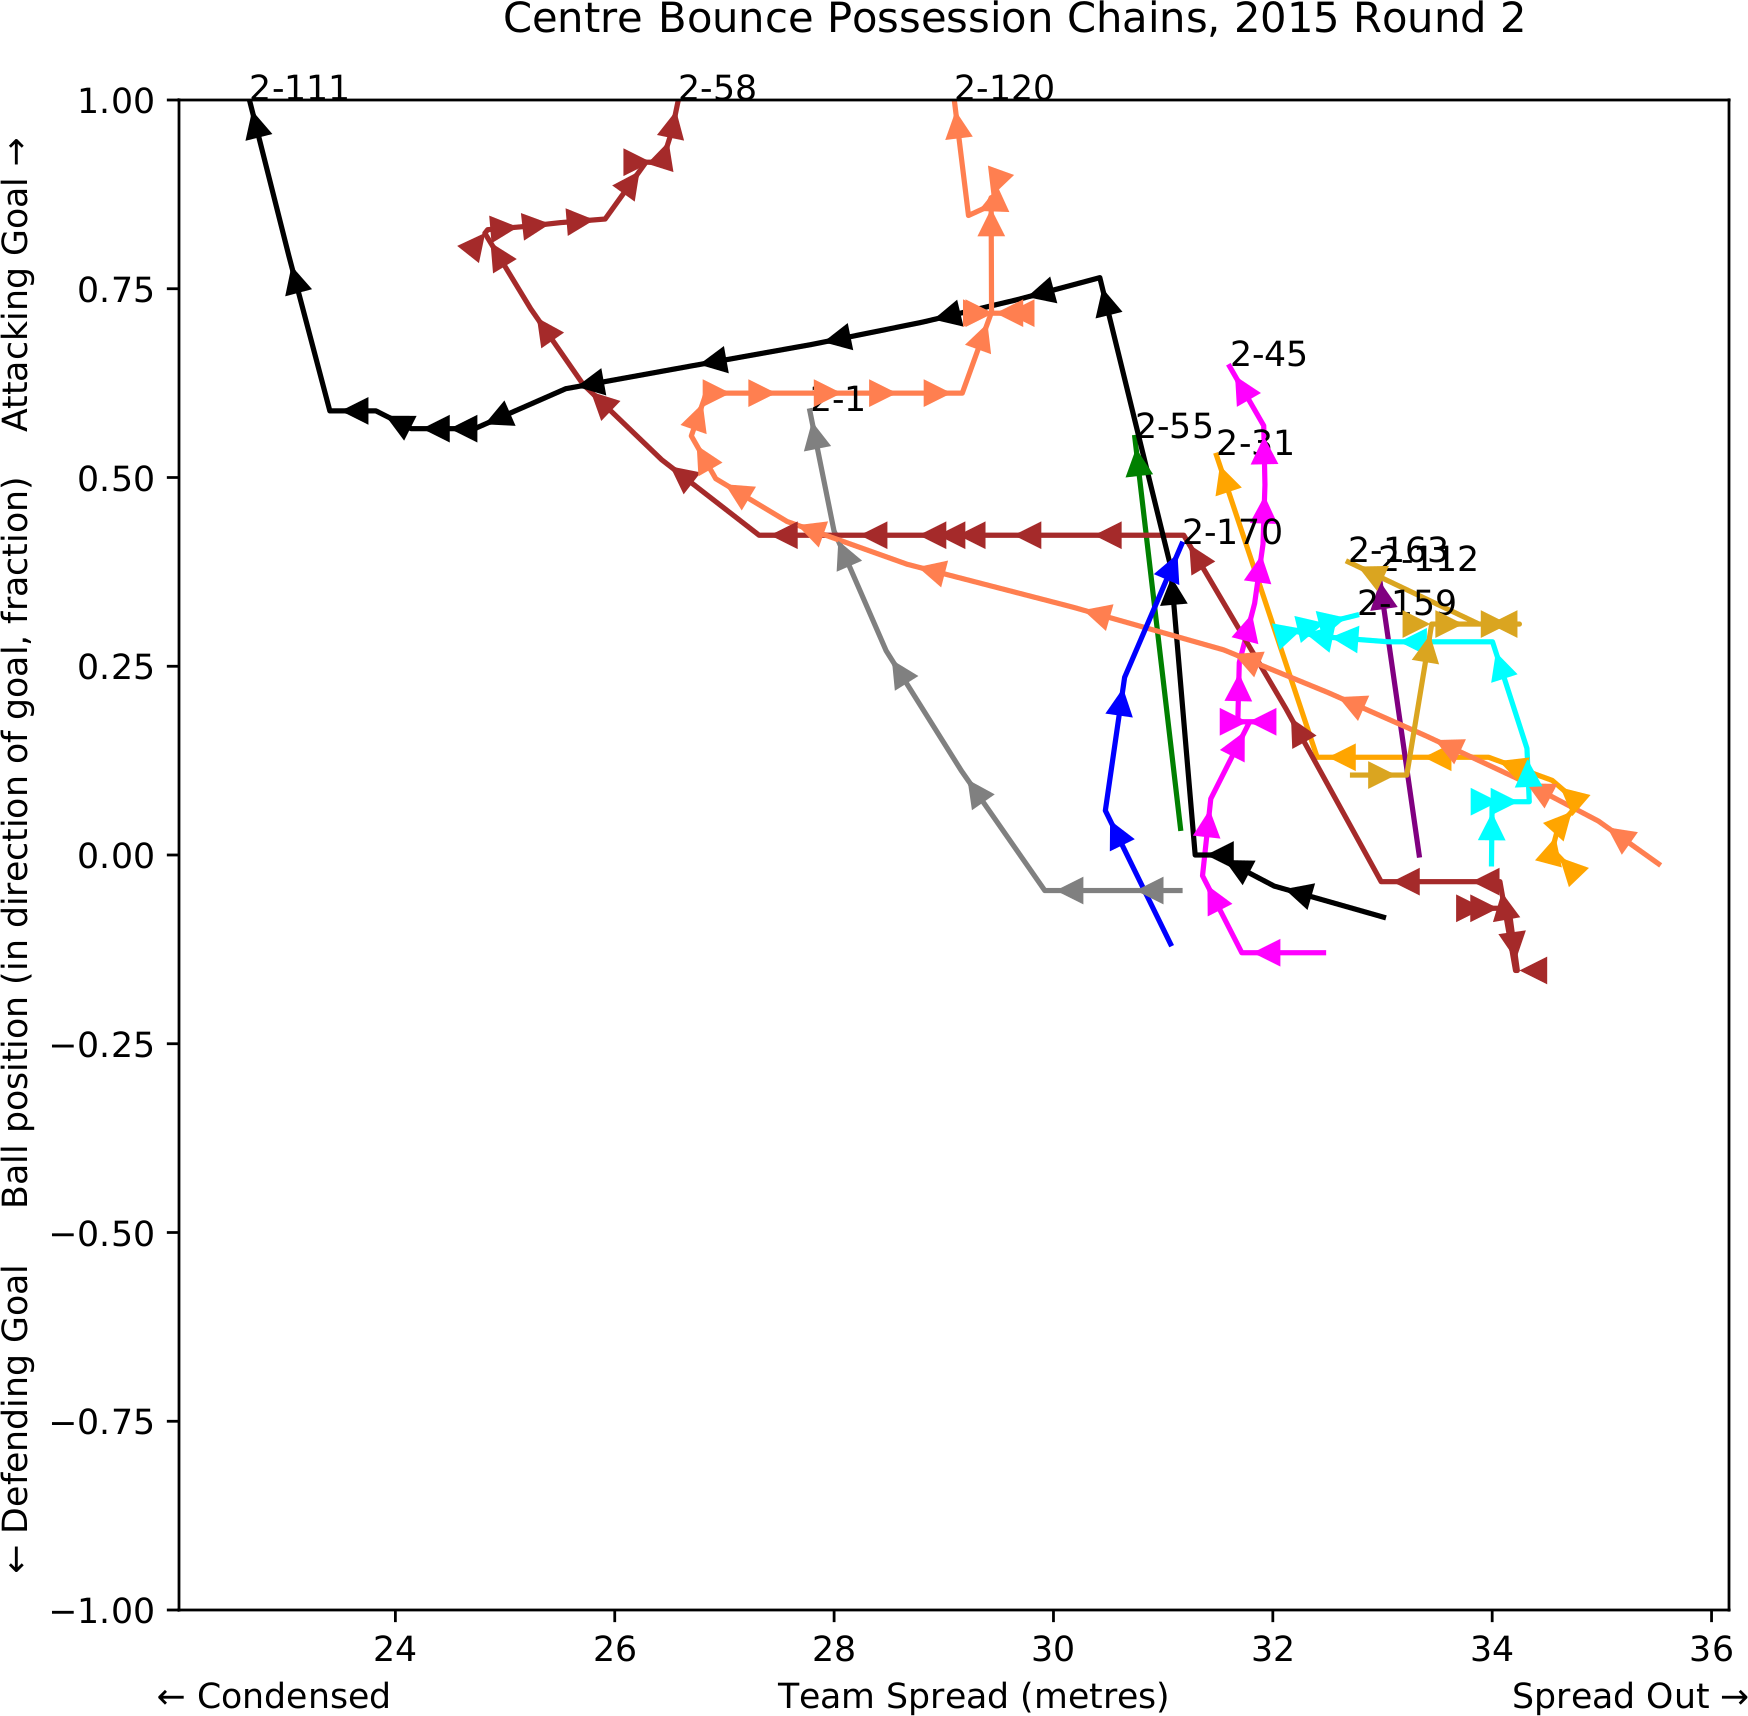
\includegraphics[width=0.9\linewidth]{figs/paper/2018-cb-r2.png}
\caption{Parametric plot of team spread and ball position for possession chains in which the analysed team successfully gained possession shortly after the \centrebounce{}. Arrows denote 1 second intervals. Chains start at the moment of possession and end when the team loses possession. Chain are labelled with the round and sequence identifier (e.g. 2-111 $\Rightarrow$ round 2, chain 111) to allow performance analysts to rapidly cross-check these with video footage. To prevent cluttering, only possession chains for one match are shown in this figure.}
\label{fig:2018-cb-r2}
\end{figure}

The parametric plots of team spread and ball position in \figref{fig:2018-cb-r2} show how the team shape at the start of play (middle-right of figure: spread > 30, ball-position = 0) changes over time as the team moves towards the goal area (top-left of figure: spread < 30, ball-position = 1.0). The plot shows that in all 3 cases where the team reached the goal area, the team condensed as they move closer towards the goal. This is to be expected, as the oval shape of the field means that when the team follows the ball they will end up packed together in a small area at the end of the oval. However, the plots show variation in the degree that the team packed together at the time of goals, which may be indicative of strategic differences.

Trace 2-111 (black) shows that after quickly advancing the ball, the team passed the ball backwards. This behaviour warrants further inspection.\footnote{In contrast to rugby, \afl{} teams are permitted to pass the ball forward, and generally do so} According to the official possession chain data, the team was considered in possession of the ball for the entire duration; however, the video shows that the team was under pressure from the opposition, and did not have clear control of the ball during this period. While moving further back from the goals is disadvantageous, the plot shows that during this time the team shape also changed and that the team emerged closer packed than before. Inspecting the GPS visualisation animations side-by-side with video confirms that prior to moving the ball backwards team members were in poor control of the ball (\figref{fig:vid-spread-before}) whereas after moving the ball backwards, the team emerged repositioned closer to the ball and regained control (\figref{fig:vid-spread-after}). This demonstrates the value of the plots in drawing attention to possible strategic advantages of reshaping the team formation that would not be evident from consideration of the ball position alone.

\begin{figure}[!htbp]
\centering
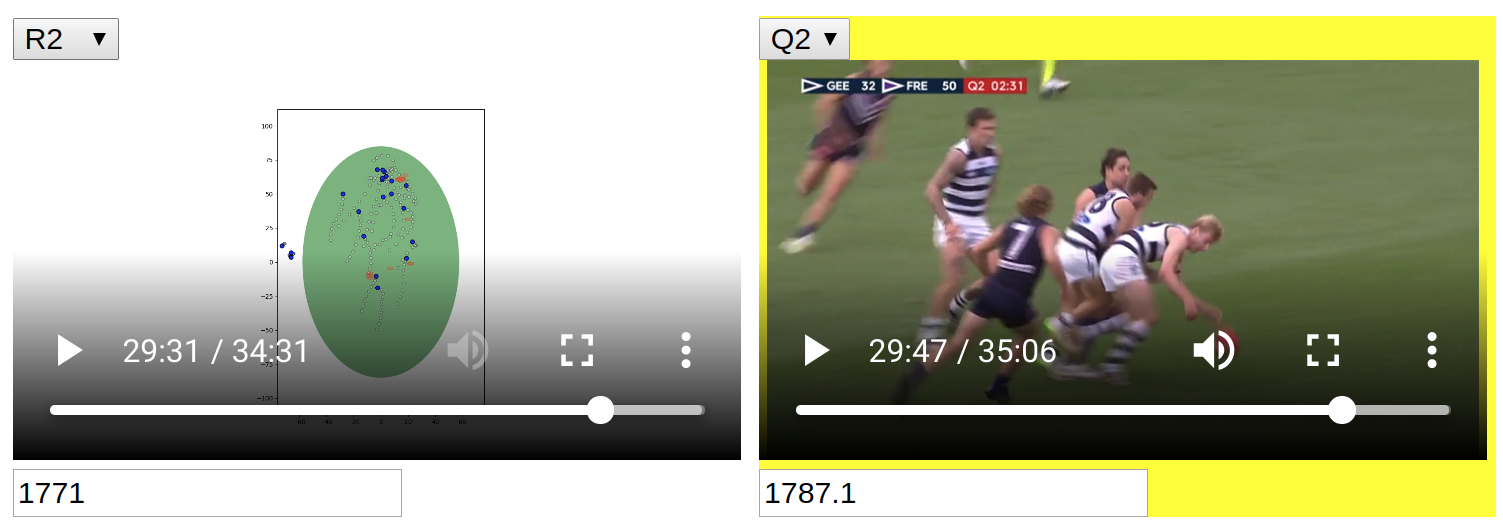
\includegraphics[width=\linewidth]{figs/paper/r2-chain-111-bad-spread.png}
\caption{Team formation visualisation side-by-side with video footage at the instant of the first turning point for chain 2-111 in \figref{fig:2018-cb-r2} where the ball was passed backward. Note the formation animation showing players trying to catch up to where the main action is occurring}
\label{fig:vid-spread-before}
% \end{figure}

% \begin{figure}[!htb]
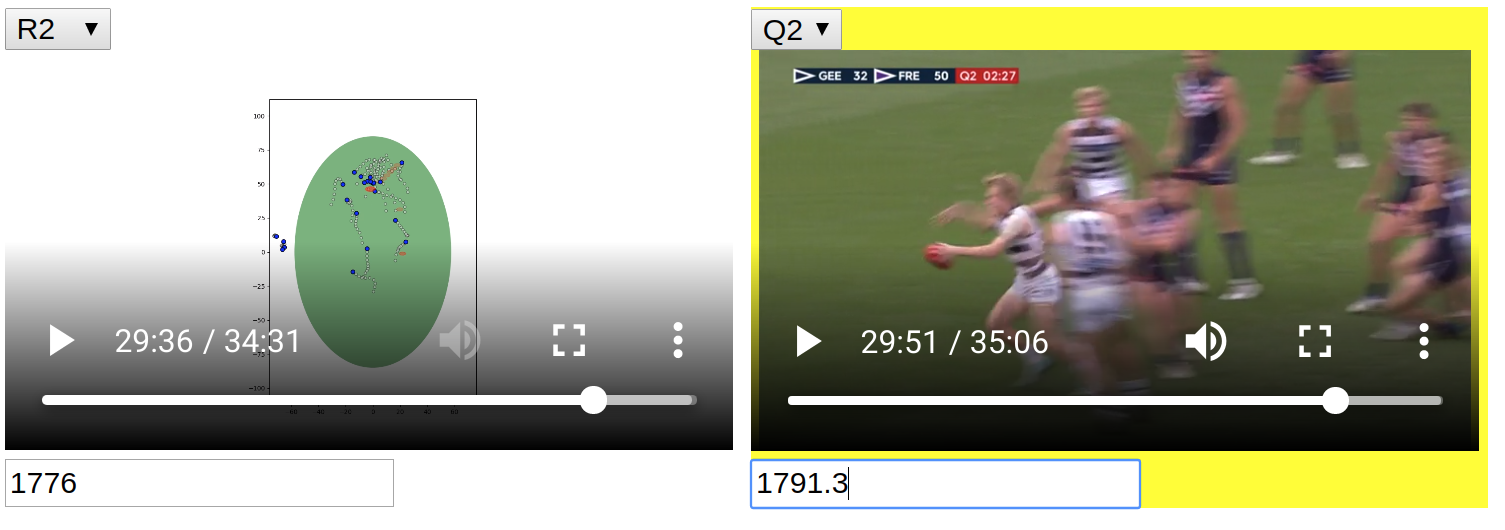
\includegraphics[width=\linewidth]{figs/paper/r2-chain-111-pass-back-but-better-spread.png}
\caption{Team formation visualisation side-by-side with video footage at the second turning point for chain 2-111 in \figref{fig:2018-cb-r2} where the team started moving the ball forward again. Note the team have reformed in a dense formation near the centre of the field where the ball has been passed to.}
\label{fig:vid-spread-after}
\end{figure}

\begin{figure}[!htb]
\centering
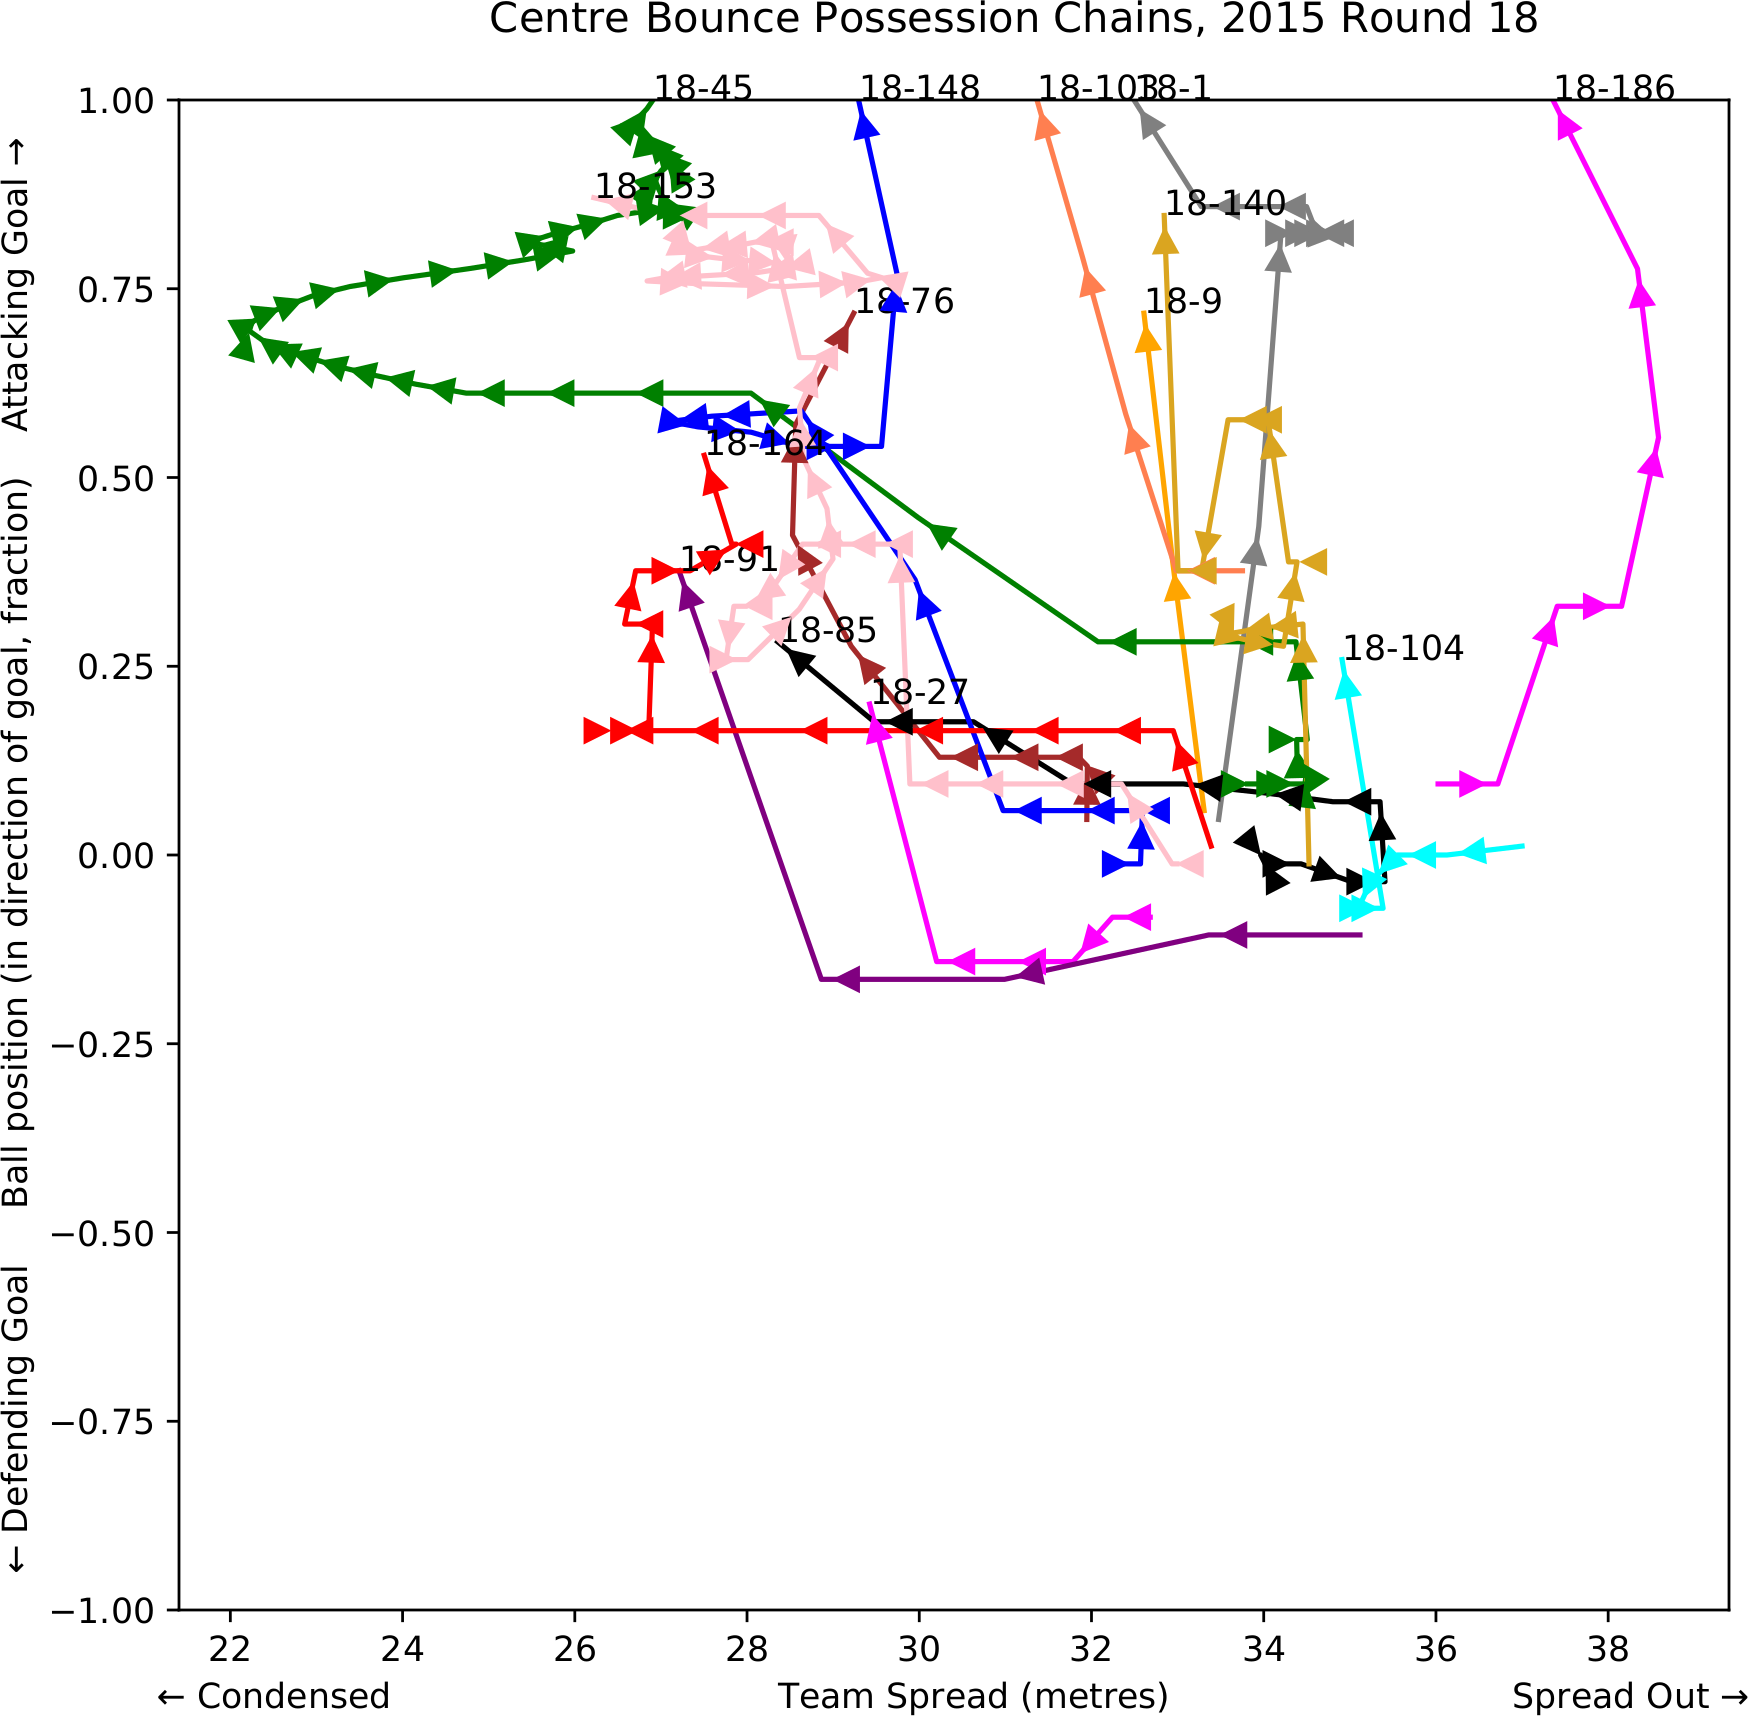
\includegraphics[width=0.9\linewidth]{figs/paper/2018-cb-r18.png}
\caption{As in \figref{fig:2018-cb-r2}, but for a match in which the team was more successful in moving the ball from \centrebounce{} directly towards the goal area}
\label{fig:2018-cb-r18}
\end{figure}

The same type of plot discussed above is shown for a different round in \figref{fig:2018-cb-r18}. Note the anomalous chain 18-186 (magenta) that shows the team spread out slightly as they headed towards goal. The long arrows denote that the ball was passed quickly towards the goal. Due to the rapid pace of ball movement, the team did not have time to follow after the ball and crowd within the goal area as they usually would. It is also possible that remaining spread out assisted the team in quickly moving the ball forward.

\subsection{Visual Comparative Analysis}

This sub-section explores data taken from possession chains over multiple matches. %rounds played at the same stadium.
Possession chains from different scenarios are overlaid on each other to visualise how formations differ between attack and defence.

\begin{figure}[!htb]
\centering
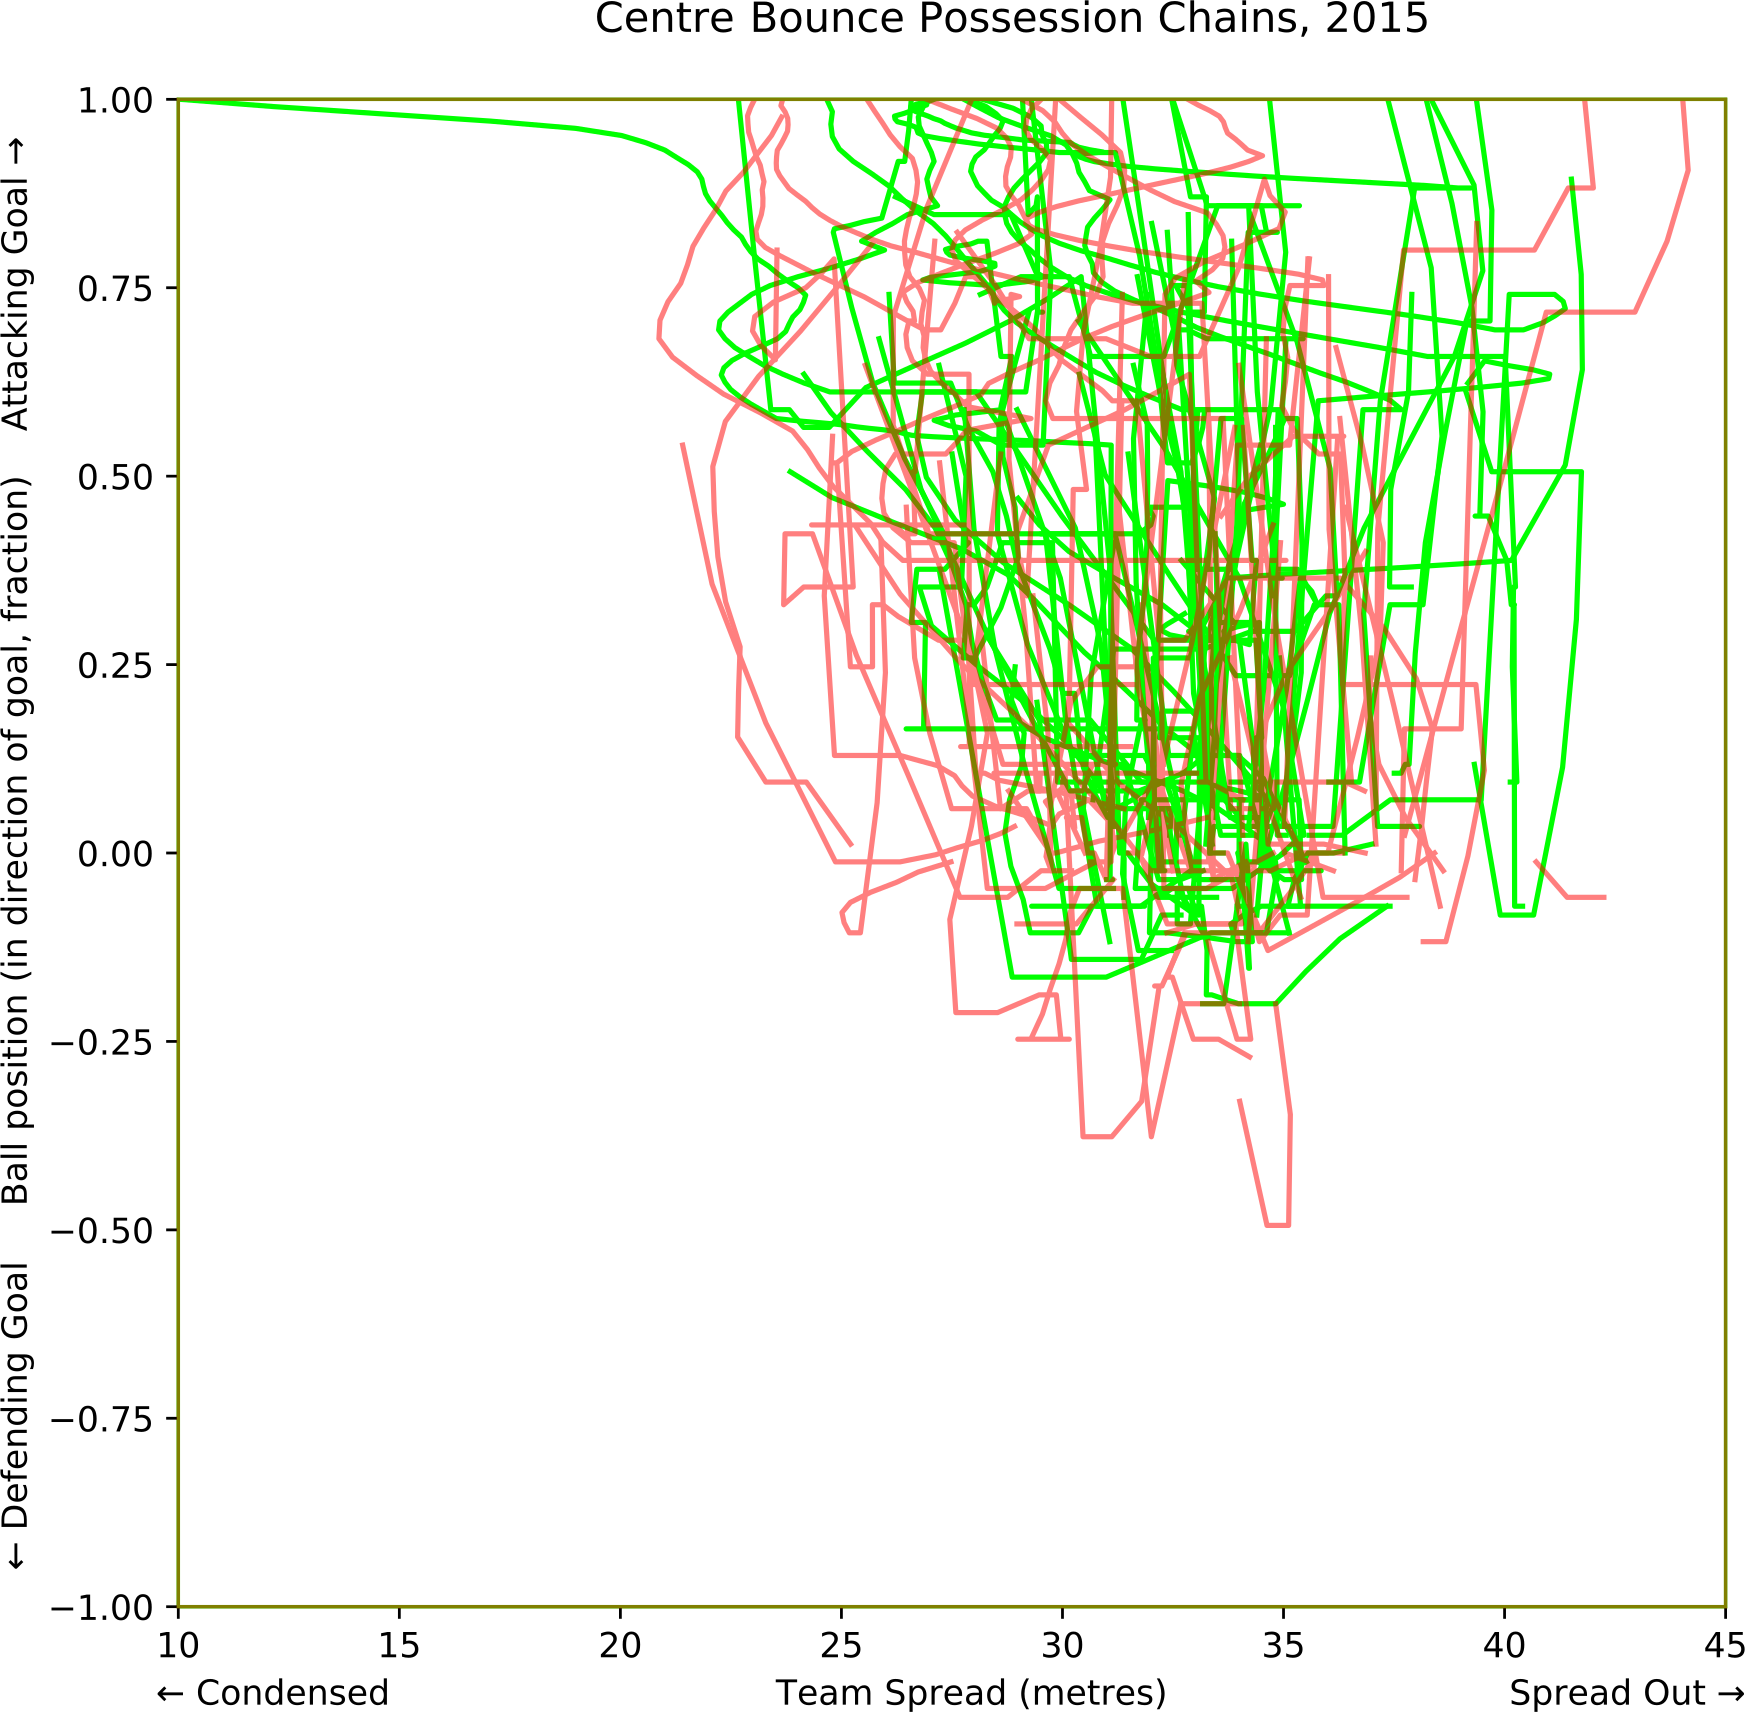
\includegraphics[width=\linewidth]{figs/paper/cb-spread-cmp-attack-and-defense.png}
\caption{Comparison of chain spread and position broken down by attack and defence phases. Attacking chains beginning with a win at \centrebounce{} are shown in green. Defending movements for opposition chains beginning with loss of the \centrebounce{} are shown in red. The direction of defending movements has been flipped for easy comparison with attacking chains.}
\label{fig:cb-spread-cmp-attack-and-defense}
\end{figure}

A comparison of attack (green) and defence (red) formations conditioned on which team wins the \centrebounce{} is shown in \figref{fig:cb-spread-cmp-attack-and-defense}. The direction during defence formations has been flipped such that defending goals during a defence phase are towards the top of the figure to align with attacking goals during the attack phase. With the exception of one anomalous attack trace (round 23, chain 69) which extends to the far left of the plot, there are no distinctive visual differences. Examining video of the anomalous trace reveals that team-mates tightly packed into the goal area during the goal attempt.

\begin{figure}[!htb]
\centering
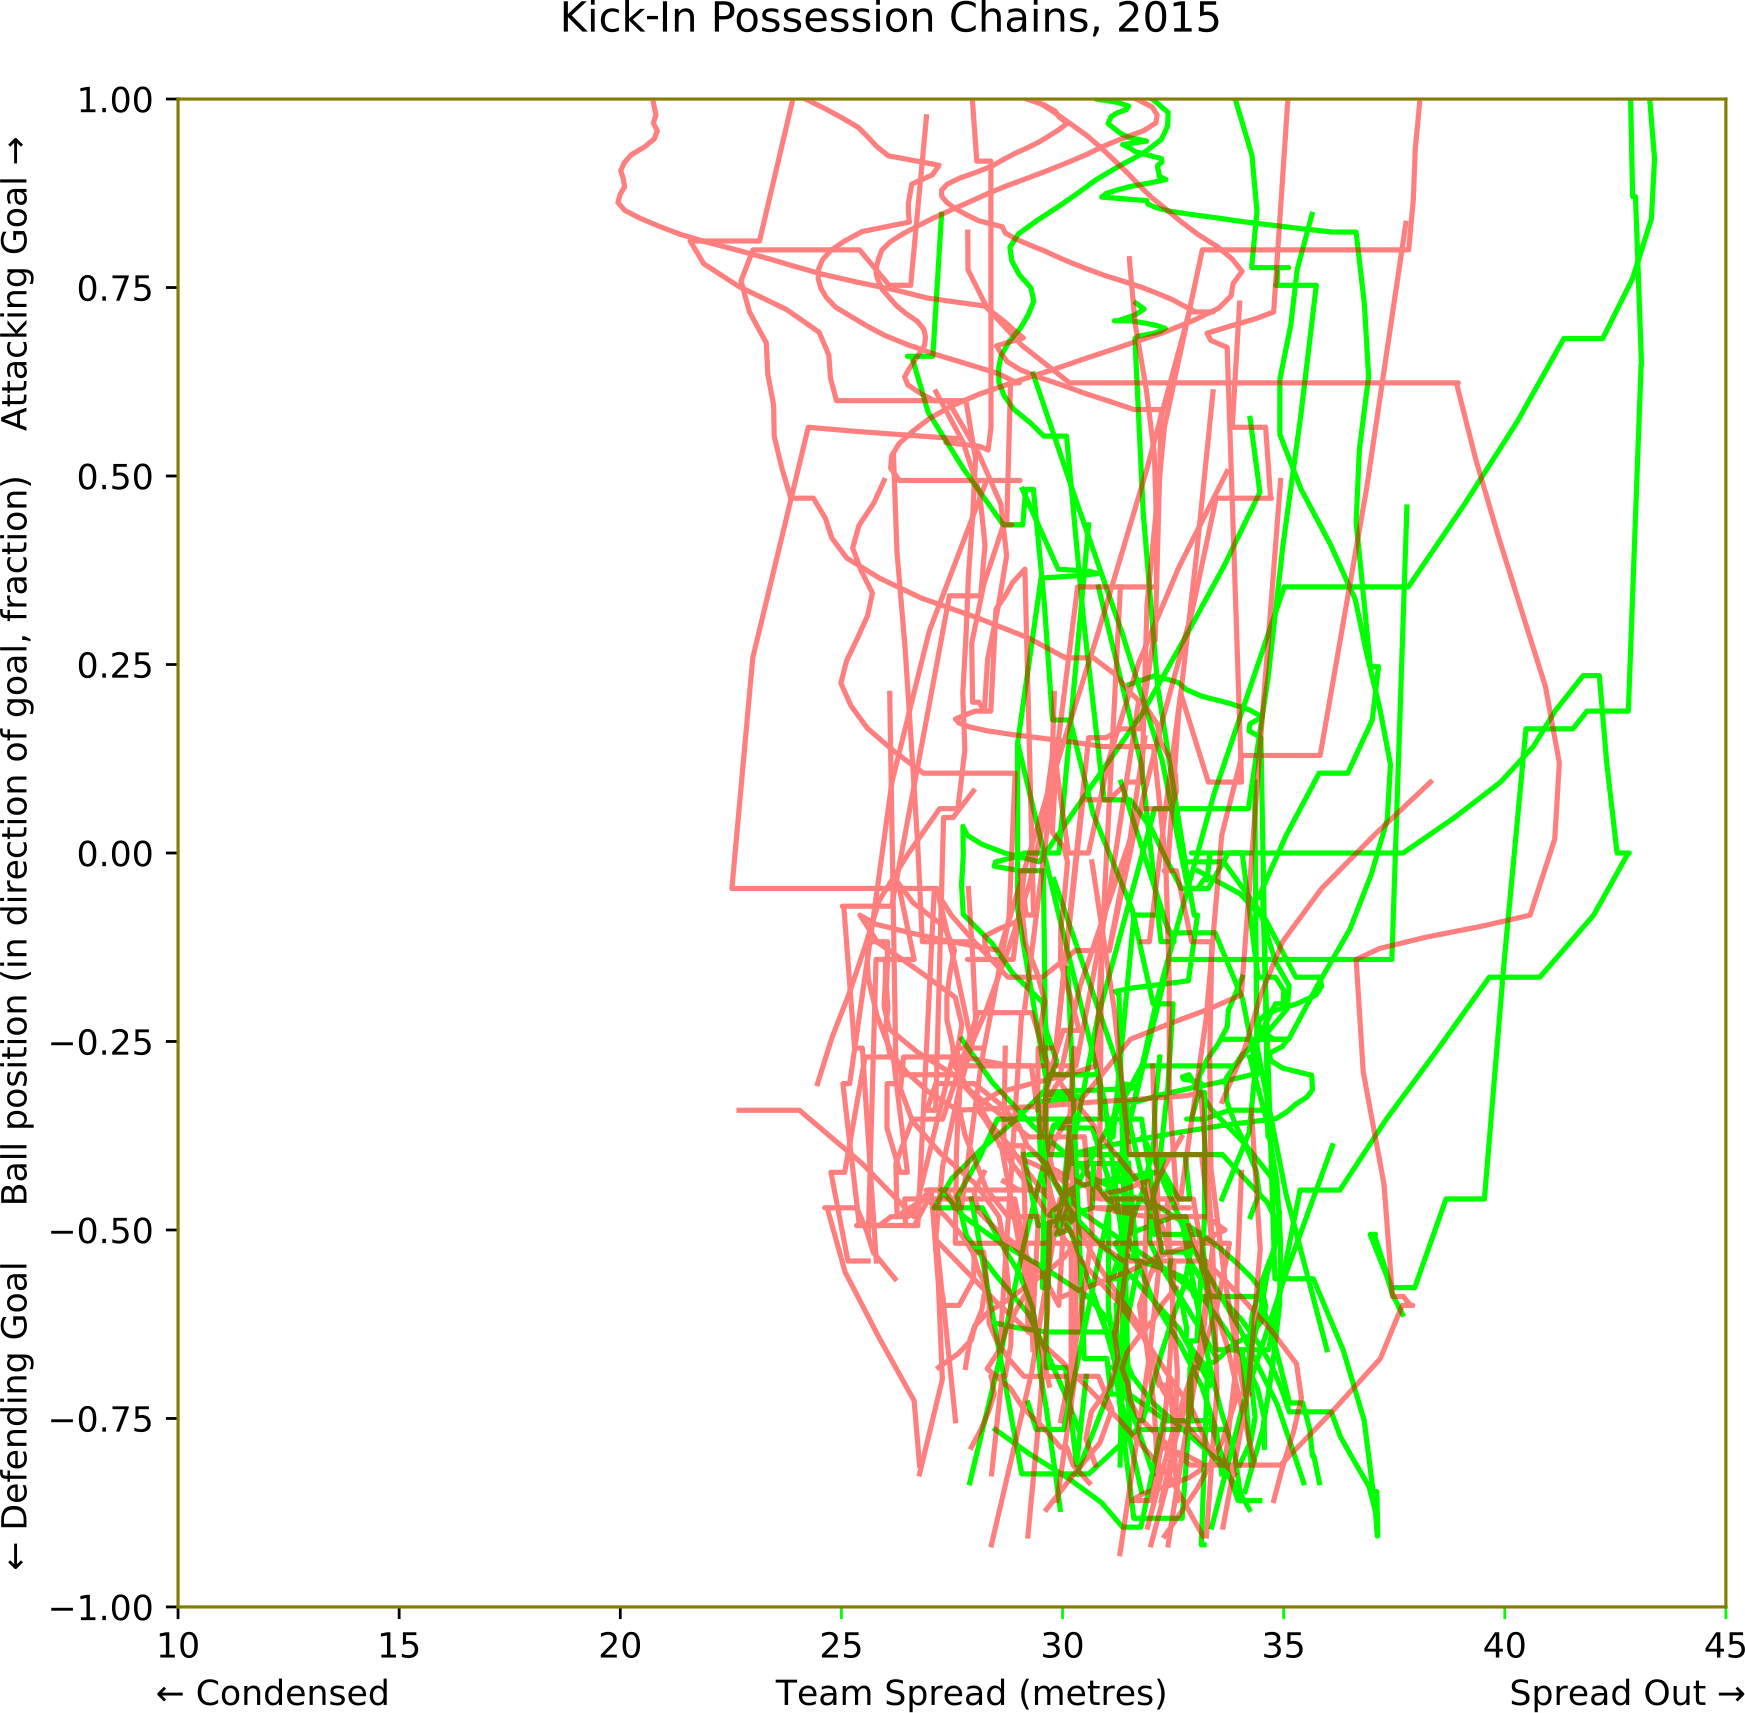
\includegraphics[width=\linewidth]{figs/paper/ki-spread-cmp-attack-and-defense.png}
\caption{As in \figref{fig:cb-spread-cmp-attack-and-defense}, but for chains beginning from a kick-in from the far side of the field.}
\label{fig:ki-spread-cmp-attack-and-defense}
\end{figure}

The same procedure was applied to compare attack (green) and defence (red) formations during kick-ins (\figref{fig:ki-spread-cmp-attack-and-defense}). Unlike the case of \centrebounces{} (\figref{fig:cb-spread-cmp-attack-and-defense}) mentioned previously, in which the situation is symmetrical for both teams until one team gains possession, in a kick-in one team is given possession at one end of the field, and must attempt to move the ball along the full length of the field past defenders to the attacking goal at the opposite end of the field. As before, the direction of defending traces were flipped so as to permit visual comparison with attack traces. It is visually apparent that the defence formations (red) tend to be more condensed than attacking formations (green), with the difference becoming more pronounced as the ball moves towards goal.

% Old: This is because when defending against a kick-off, the defending team is sandwiched between the attackers and the goal they are defending.
% D.H.: Suggested that perhaps it is because defending team doesn't bother (conserves energy) chasing ball if the opposition breaks through.
% Conclusion: Let's avoid mixing interpretation with results. Examining 18-133, 18-71 (the two most extreme cases), it seems that at end the opposing team had been awarded possession (e.g. a free kick) and thus Geelong had plenty of time to position themselves to defend. Geelong might be slightly more condensed when defending than attack because don't have anyone tagging the kicker.

\subsection{Quantitative Analysis}

This sub-section quantifies the visual observations made in the preceding sub-sections.

\subsubsection{Quantifying Team Spread in Attack versus Defence}

\begin{figure}[!htb]
\centering
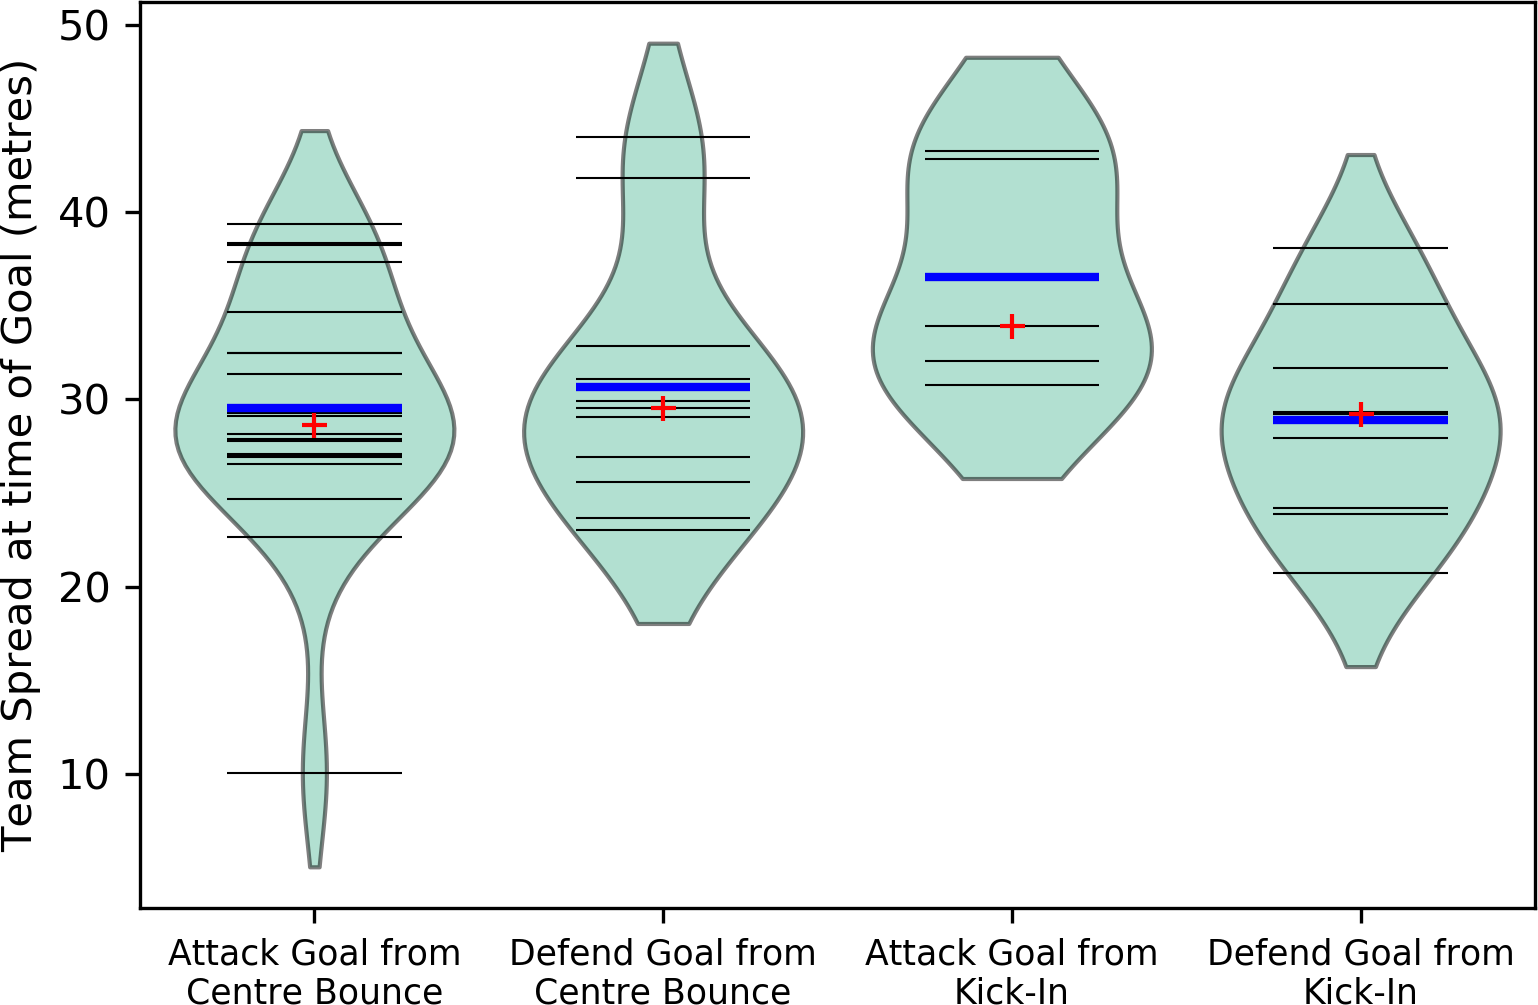
\includegraphics[width=0.9\linewidth]{figs/paper/spread-vs-type.png}
\caption{Violin plots showing the density distribution of spread at the time the ball reaches the goal area. From left to right: chains beginning with won \centrebounce{}; movements during opposition chains beginning with lost \centrebounce{}; chains beginning with team kick-in from far side of field; movements during opposition chains beginning with opposition kick-in. Each black line corresponds to a possession chain that reached the goal area and marks team spread at the time of goal (or team spread at the time of conceding a goal when defending). Blue lines denote the mean, and red pluses (+) denote the median.} % TODO: Fix labels in diagram. % https://www.statsmodels.org/dev/generated/statsmodels.graphics.boxplots.beanplot.html
\label{fig:spread-vs-type}
\end{figure}

Violin plots showing the density distribution of team spread at the time the ball reaches the goal area are shown in \figref{fig:spread-vs-type}. Values of the mean and standard deviation for each group are reported in Table~\ref{tab:spread-groups}. Prior to conducting further statistical tests, Shapiro-Wilk tests were performed to validate the assumption of normality, which held for all groups ($p > 0.05$) with the exception of the Attack Goal from Centre Bounce group ($p = 0.04$) due to an outlier\footnote{Note the anomalously low value of team spread (10 metres) occurring in the Attack Goal from Centre Bounce group due to an instance where the team packed closely together near the goal area. Re-running the Shapiro-Wilk test without this outlier indicates the group is consistent with the assumption of normality ($p = 0.12$).}. To test the hypothesis that team spread would change in attack versus defence, Welch's \textit{t}-tests\footnote{Unlike Student's \textit{t}-test, Welch's \textit{t}-test does not assume equal variance.} were performed to test the significance of difference between attack spread versus defence spread, controlling for the location of initial ball possession (centre bounce/kick-in). Examining team spread at the time of goal following a \centrebounce{}, there was no statistically significant difference between the group of cases where the team was defending and group of cases where the team was attacking\footnote{The difference is not statistically significant regardless of whether the outlier is included in the calculation or not.} ($p > 0.05$). Examining team spread at the time of goal following a kick-in, the team is more spread out during an attack on goal than when defending against an attack on goal. This result is weakly statistically significant ($p < 0.05$). Details of the \textit{t}-tests are reported in Table~\ref{tab:ttest-details}.

% All statistical tests were conducted using the SciPy\footnote{[Software] Jones E, Oliphant E, Peterson P, et al., ``SciPy: Open Source Scientific Tools for Python'', 2001-2019. \url{https://scipy.org/}} statistics library for Python.

%  This is preferable to the discredited two step approach of running Levene's test of homoscedasticity followed by Student's \textit{t}-test
% https://stats.stackexchange.com/questions/289449/is-variance-homogeneity-check-necessary-before-t-test
% - https://onlinelibrary.wiley.com/doi/abs/10.1348/000711004849222 "A note on preliminary tests of equality of variances" (2004) [zimmerman2004-stat-testing]
%
% "Optimum protection is assured by using a separate‐variances [e.g. Welch's t-test] test unconditionally whenever sample sizes are unequal."
%
% https://www.ncbi.nlm.nih.gov/pmc/articles/PMC3693611/#A3505R2 - Normality Tests for Statistical Analysis: A Guide for Non-Statisticians -- Recommends Shapiro-Wilk test

% Welch's \textit{t}-test is similar to Student's \textit{t}-test, but does not require that groups have equal variance.
% Unlike Student's \textit{t}-test, Welch's \textit{t}-test does not assume equal variance.}

\begin{table}[htpb]
\caption{Team spread statistics for attack/defence at the time instant the ball reaches the goal area for possession chains starting from centre bounce/kick-in. Table corresponds to visual presentation of data in \figref{fig:spread-vs-type}. N denotes number of possession chains of the specified type that reached the goal area. $\mu$ denotes the mean (i.e. the expected team spread at the time the ball reaches the goal area). $s$ denotes the sample standard deviation (i.e. an indicator of whether the team spread is consistent at the time the ball reaches the goal area across multiple possession chains).}
\label{tab:spread-groups}
\begin{tabular}{lrrr}
\toprule
                & \multicolumn{1}{c}{N}  & \multicolumn{1}{c}{$\mu$ (metres)}      & \multicolumn{1}{c}{$s$ (metres)}      \\
\midrule
Attack Goal from Centre Bounce & 20 & 29.57 & 6.67 \\
%cb\_score\_corr & 19 & 30.599823 & 4.963848 \\
Defend Goal from Centre Bounce & 11 & 30.68 & 6.78 \\
Attack Goal from Kick-In & 5  & 36.57 & 6.03 \\
Defend Goal from Kick-In & 9  & 28.91 & 5.54 \\
\bottomrule
\end{tabular}
\end{table}

% https://docs.scipy.org/doc/scipy/reference/generated/scipy.stats.ttest_ind.html
\begin{table}[htpb]
\caption{Welch's \textit{t}-test results showing significance of difference of team spread at time of attacking goal ($\mu_{A}$) versus team spread at time of defending goal ($\mu_{D}$). $t$ and $p$ denote the \textit{t}-statistic and two-tailed \textit{p}-value reported by Welch's \textit{t}-test (carried out using SciPy 1.2.1). Significant results marked with a star (*).}
\label{tab:ttest-details}
\begin{tabular}{lrrl}
\toprule
                                  & $\mu_{A} - \mu_{D}$      & \multicolumn{1}{c}{\textit{t}} & \multicolumn{1}{c}{\textit{p}} \\
\midrule
Attack vs. Defend Goal from Centre Bounce & -1.11 & -0.44    & 0.66  \\
Attack vs. Defend Goal from Kick-in       & 7.66  & 2.34     & 0.05*  \\ % Fixed to report Welch's t-test rather than standard independent 2 sample test.
\bottomrule
\end{tabular}
\end{table}

\subsubsection{Quantifying Relationship between Game Speed and Team Spread}

\begin{figure}[!htb]
\centering
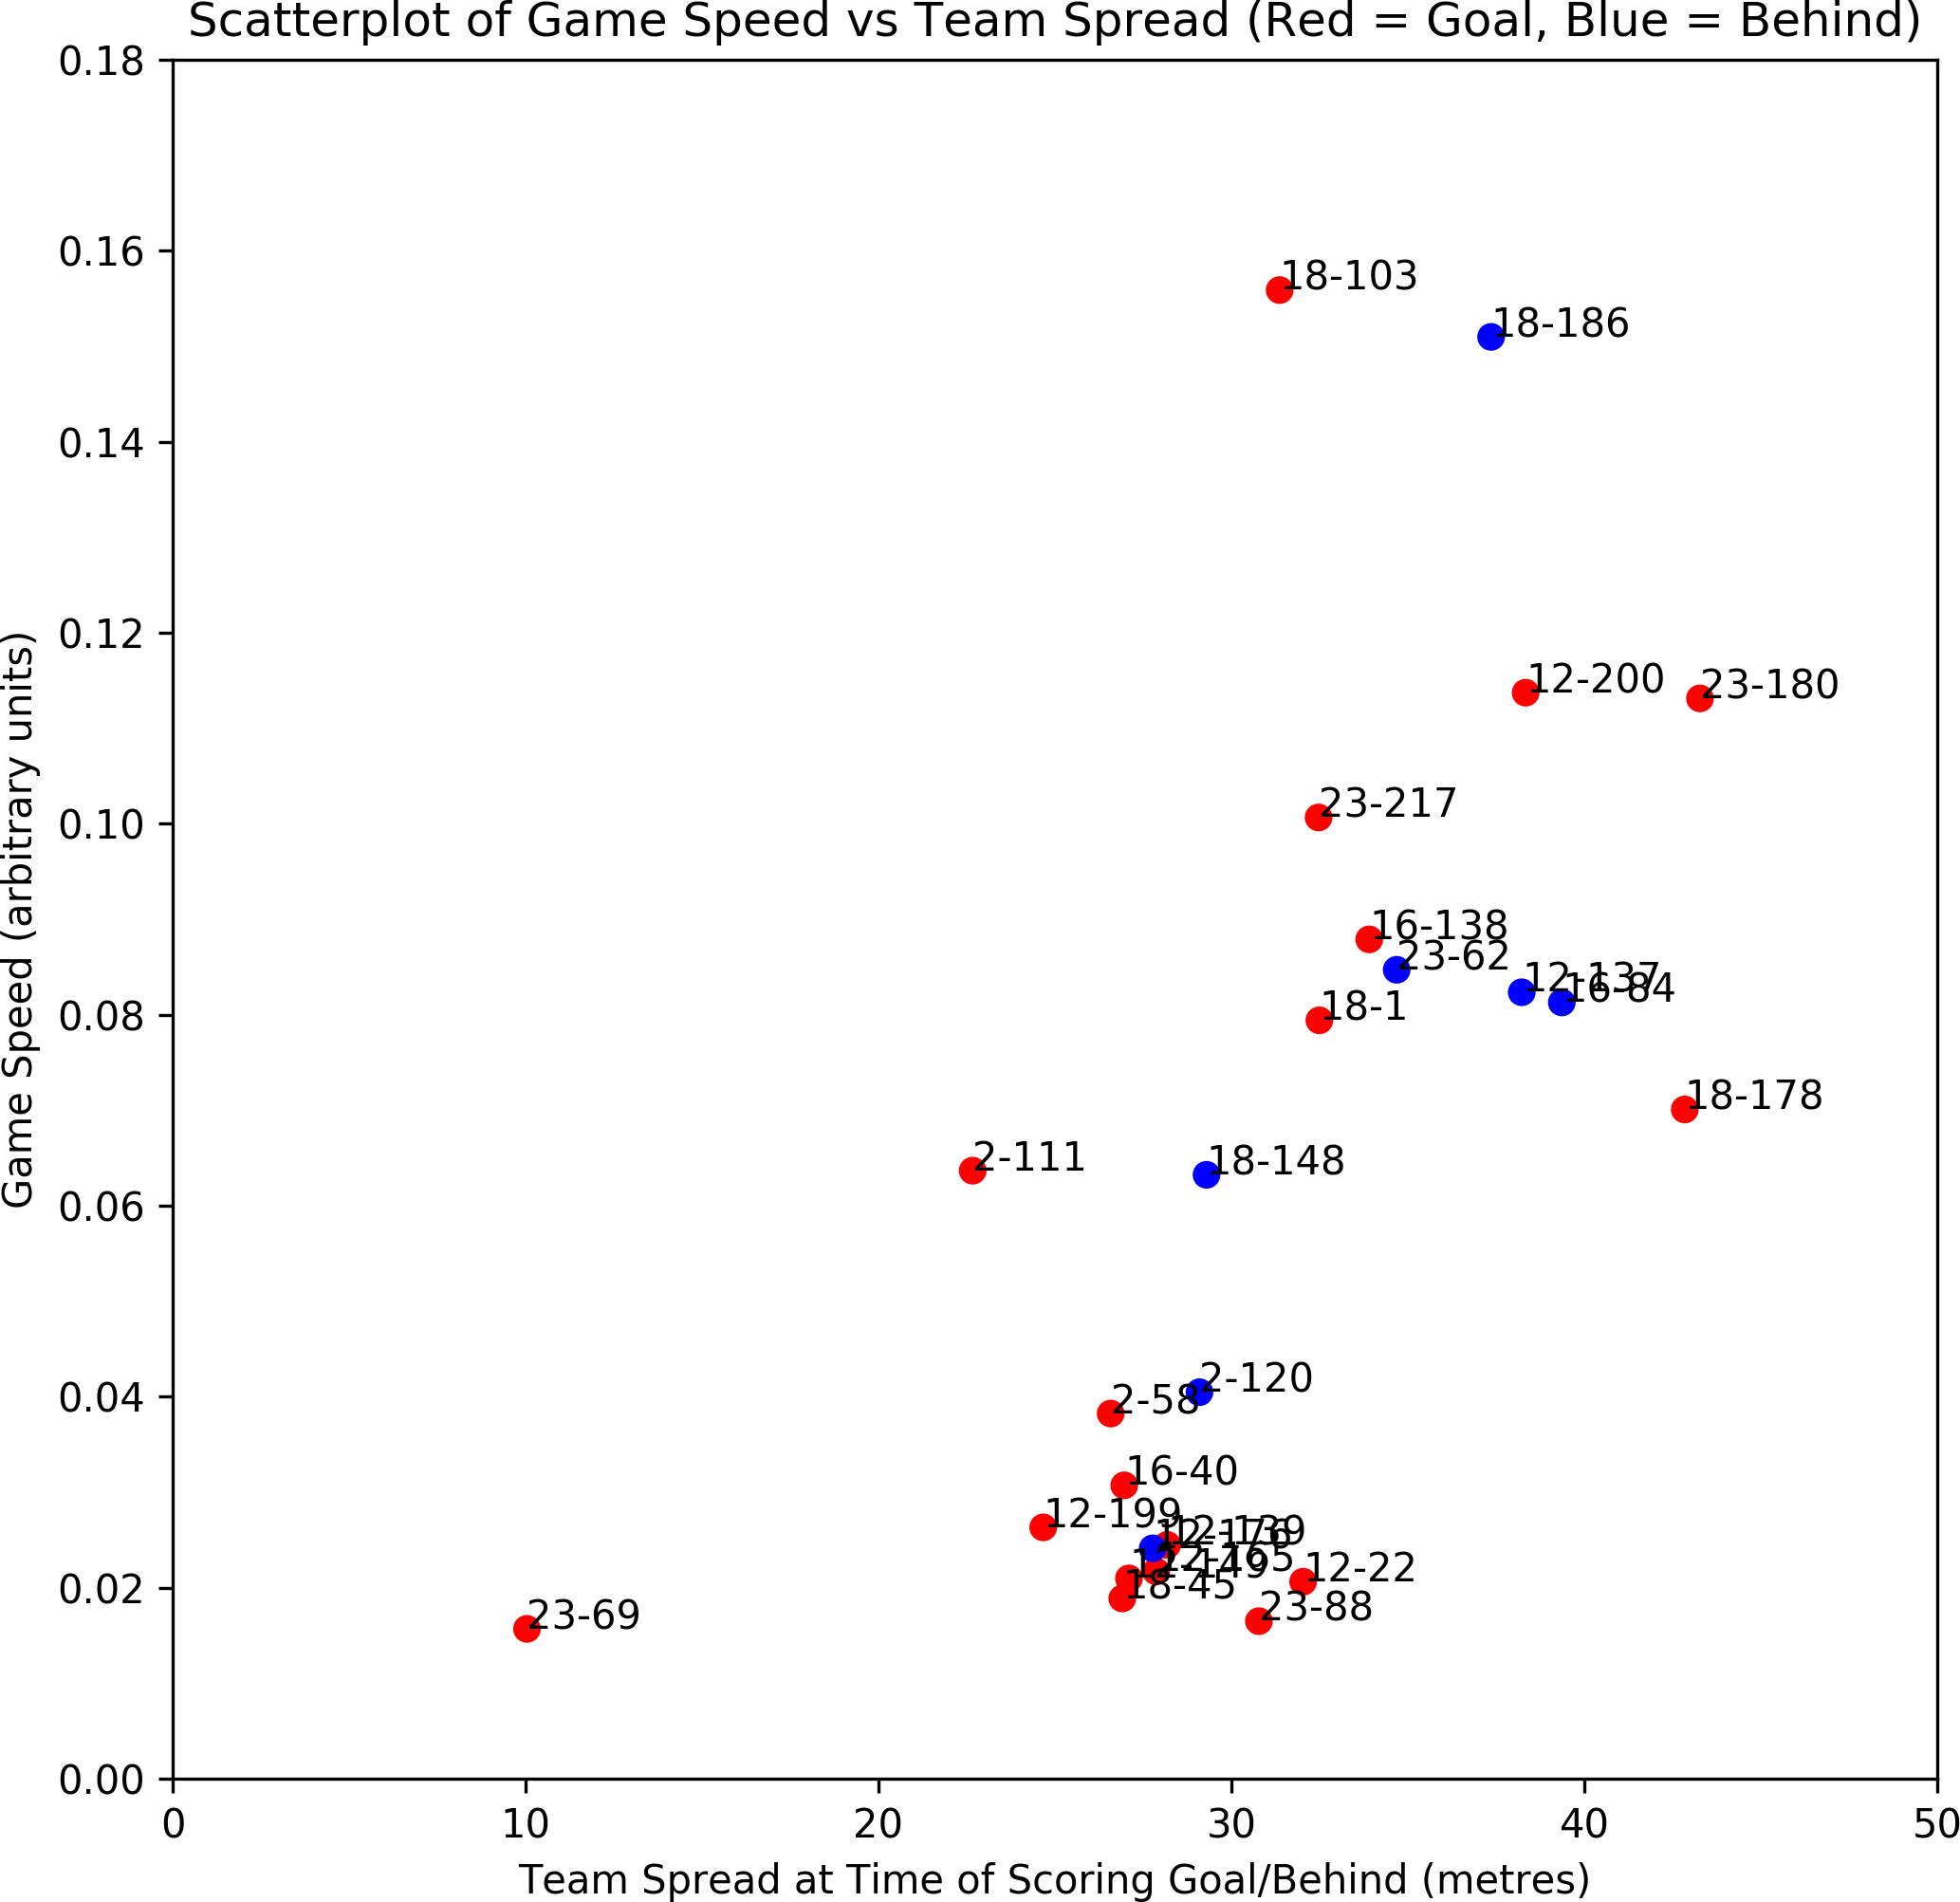
\includegraphics[width=0.8\linewidth]{figs/paper/speed-vs-spread-succeed.png}
\caption{Scatterplot of game speed versus team spread (at time of scoring). Combines data from chains beginning with team possession at \centrebounce{} and chains beginning with team possession at kick-in. Red dots indicate spread and average game speed at time of goal. Blue dots indicate a behind (missed goal). Labels denote the match and chain identifier so that performance analysts can cross-check anomalous chains with video footage.}
\label{fig:speed-vs-spread-attack}
\end{figure}

\begin{figure}[!htb]
\centering
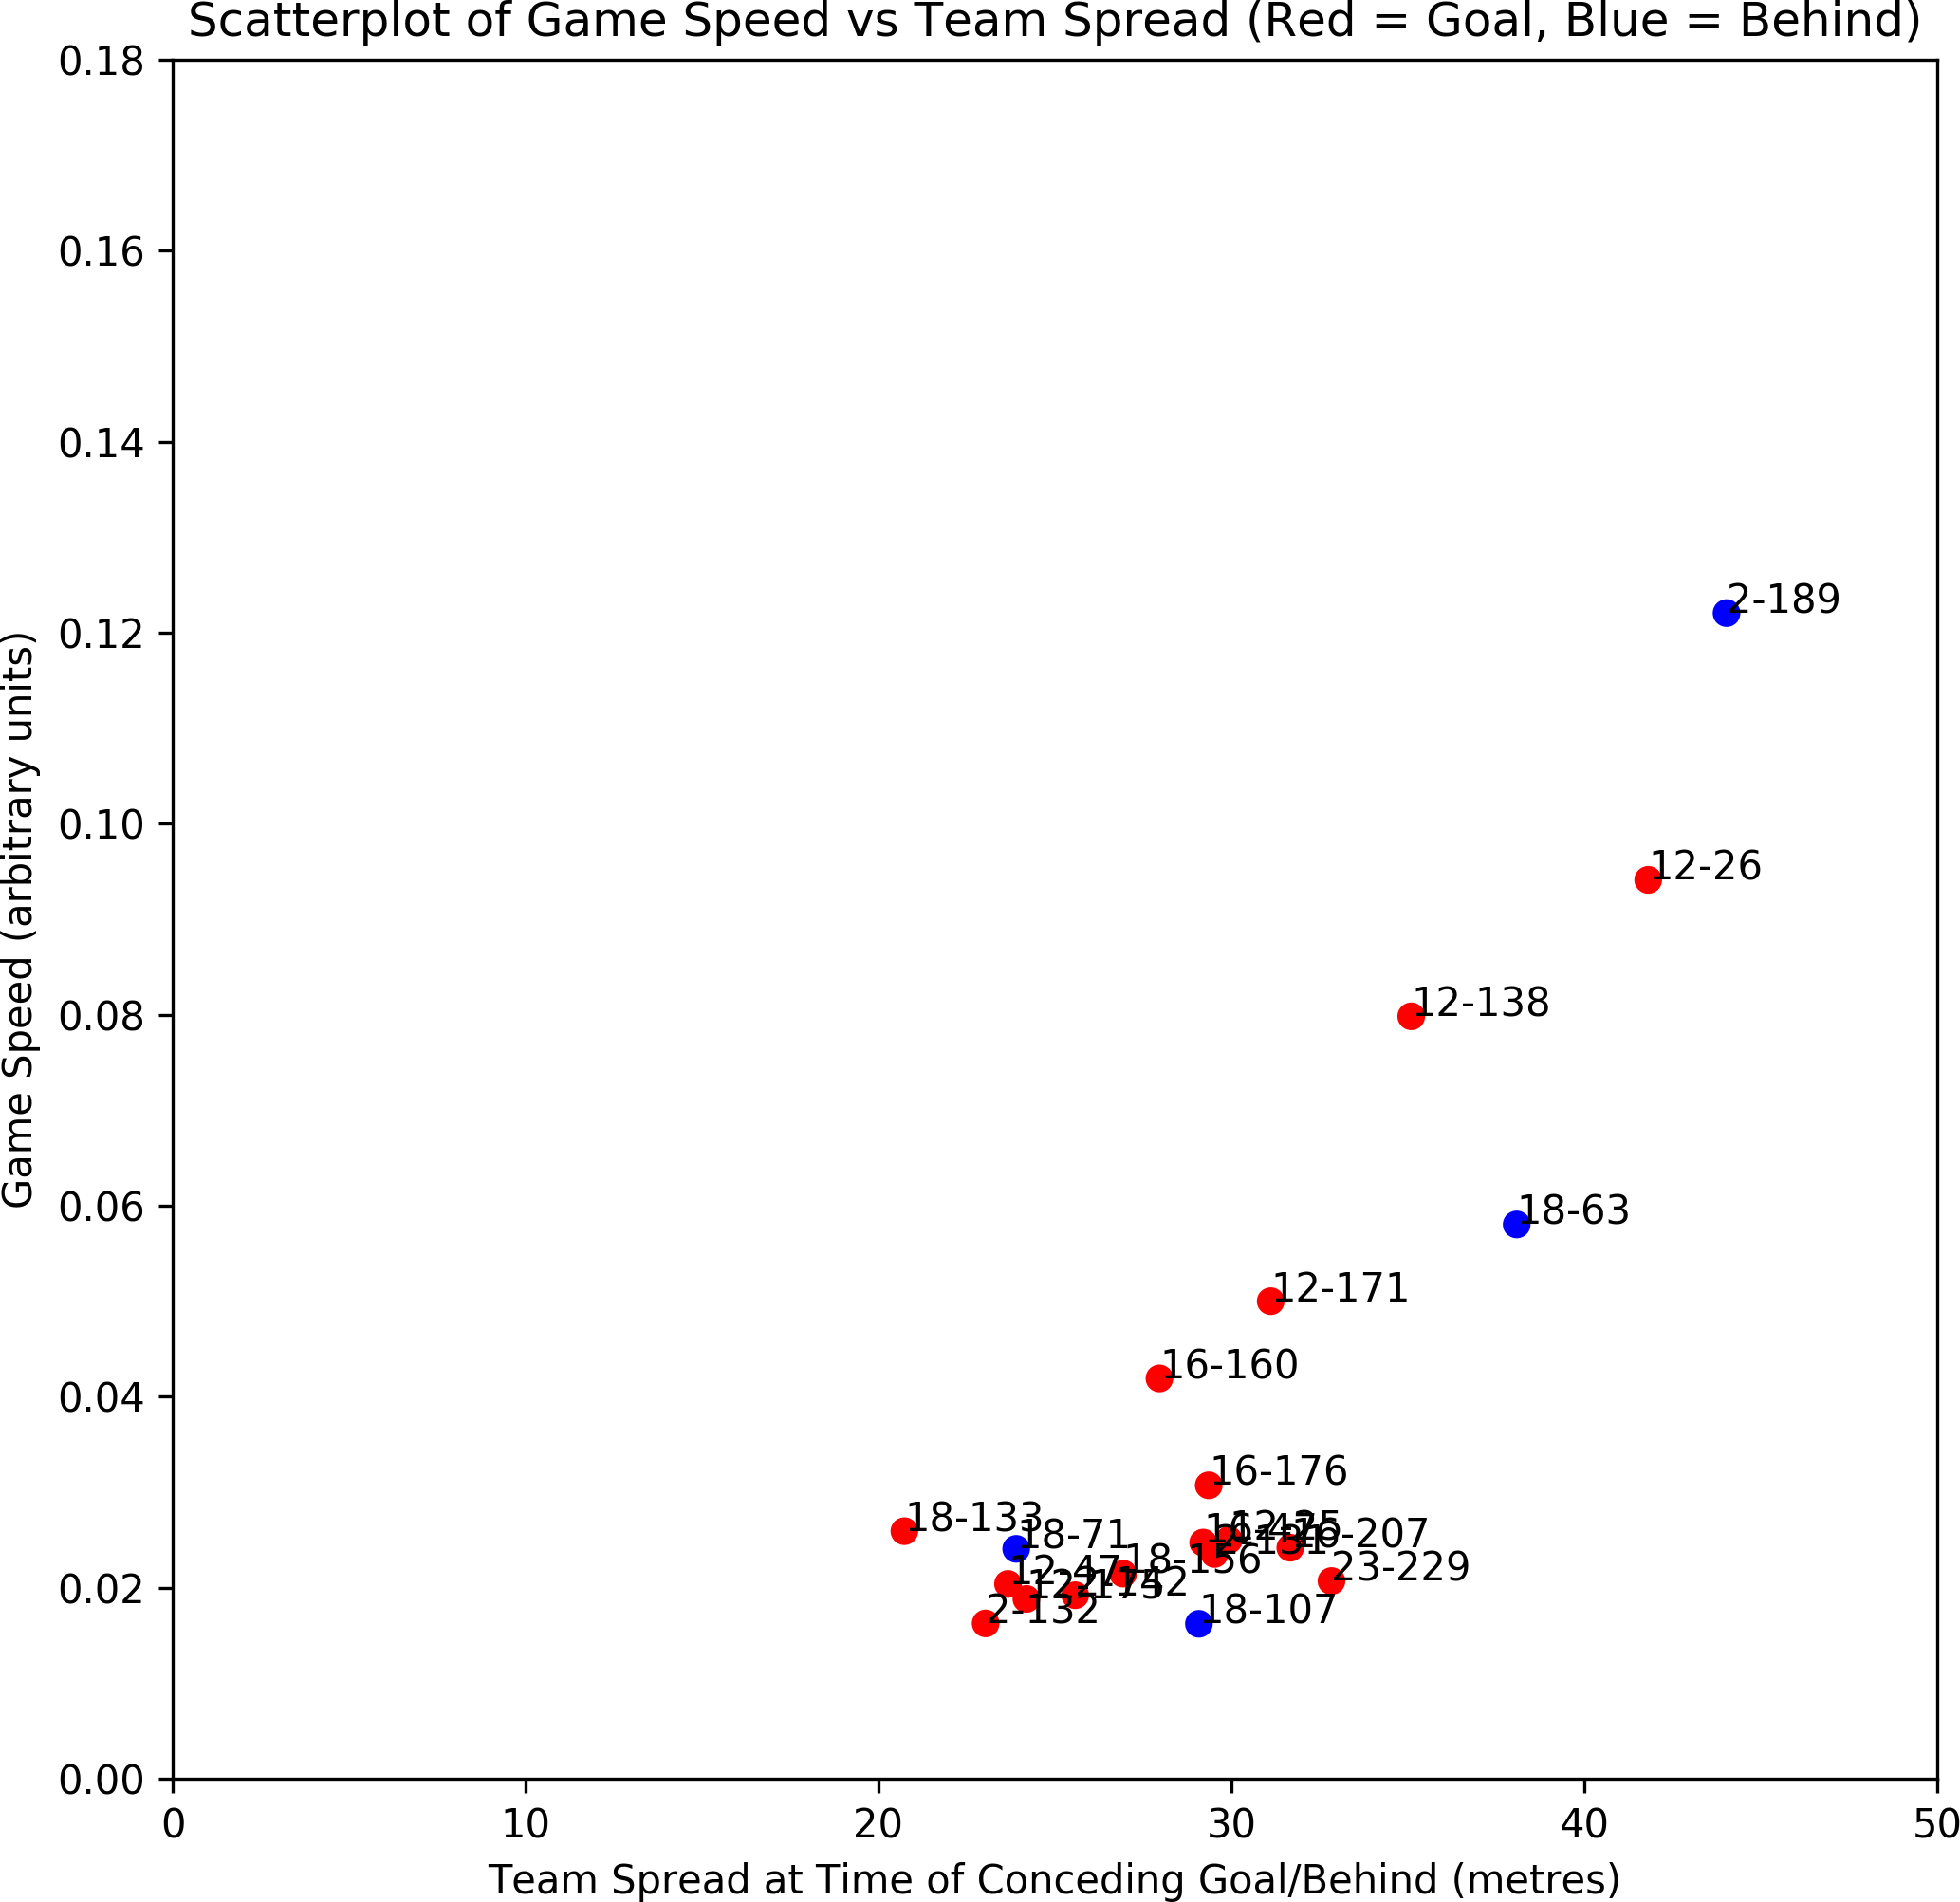
\includegraphics[width=0.8\linewidth]{figs/paper/speed-vs-spread-concede.png}
\caption{As in \figref{fig:speed-vs-spread-attack}, but analysing game speed versus team spread for defence at time of goal by opposition team.}
\label{fig:speed-vs-spread-defence}
\end{figure}

%\todo{WRONG TEAM!!! (need to regen for attack, not defence)} %Fixed

As a result of the exploratory analysis, it was hypothesised that the team being spread out is associated with quick forward ball movement. To test this hypothesis, the following variables were utilised: the team spread; the forward distance the ball moved (e.g. a \centrebounce{} to goal only has to cover half the field, whereas a kick-in to goal has to cover the full length of the field); and the duration of the possession chain. \textit{Game speed} was then defined as the forward distance\footnote{Only the displacement vector between the position at the time of initial possession of the ball and the position at the time of losing possession was considered, as opposed to the total path length. Furthermore, only the component of the displacement vector in the direction of goal heading was used. This means the forward distance metric will be less than the total path distance covered by the player. However, this is sufficient for the analysis, as the analysis is primarily concerned with game speed ratios rather than measuring physical ball speed.} divided by time. An increasing relationship was found between team spread and game speed when attacking goal, corresponding to the data displayed in \figref{fig:speed-vs-spread-attack} (Pearson's~$r = 0.61$, $p < 0.05$; Spearman's~$\rho = 0.69$, $p < 0.001$). A strong linear relationship was found between team spread and game speed when defending goal, corresponding to the data displayed in \figref{fig:speed-vs-spread-defence} (Pearson's~$r = 0.85$, $p < 0.001$; Spearman's~$\rho = 0.66$, $p < 0.01$).

\subsection{Discussion}

In communication with analysts at the club that provided the data, they explained that, in principle, teams try to spread out for a good attack to get around the defence, and condense in a good defence. However, when examining possession chains that begin with a \centrebounce{}, there was no significant difference observed between team spread during attack and defence. This may be explained by AFL players defending by ``tagging'' (following after) a player of the opposite team. When examining kick-ins, there was weak evidence to suggest that the team spread out more when attacking from a kick-in than when defending from a kick-in. The club suggested that this may be explained by a ``zone defence'' strategy (protecting space rather than following after an opponent) employed in scenarios when the team has sufficient time to set up a defence.

There may be some misalignment of the club analysts' conception of spreading out, and the mathematical definition of spread used in this thesis. There are multiple ways that these notions could be formalised, thus future work is needed to explore alternative mathematical definitions of spread that more closely align with the tacit definition used by sport practitioners. For example, if a player is injured or fatigued, they may remain on-field for a short period, but may stay still rather than moving with the rest of the team formation, thus should ideally be removed from the team spread calculation.

% Club provided example of injured player on field that does not move with the rest of the team.

There is a strong correlation between team spread and game speed; however, caution is needed in the interpretation of this relationship. It is possible that spreading out helps the team move the ball forward quicker; however, a more likely explanation is that when the team moves the ball forward quickly, they do not have time to reform into a unified attacking formation as they would when they move the ball slowly forward. To definitively test for a causal relationship would require an intervention study to vary a single variable at a time. If causality can be established, then understanding this relationship would allow teams to control the game speed. While this study was unable to establish whether a certain team spread or game speed is desirable\footnote{From the exploratory analysis, up until the point that a turnover occurs, there does not appear to be any visually apparent distinction between chains that end short, and chains that are successful. Furthermore, the behinds (blue) highlighted in \figref{fig:speed-vs-spread-attack} appear to be distributed similarly to goals (red) in terms of both spread and game speed, indicating that goal accuracy is independent of these factors.}, knowledge of which formations speed up or slow down the game could have strategic implications when only a short time remains before the end of the quarter.

\subsection{Conclusions}

This thesis section demonstrated an approach to utilising GPS data for the purpose of strategic analysis of \afl{} teams. It demonstrated the value of GPS data as a tool to form hypotheses, identify patterns, investigate anomalies, and quantitatively test performance analysts' assumptions about the game.

Caution is advised in the utilisation of specific findings. The difference between attacking and defending formations for kick-ins was only weakly significant; however, the observation that teams generally spread more in attack than in defence appears to be in alignment with Alexander et al.'s preliminary findings \cite{Alexander2019a, Alexander2019b}. While there is a strong correlation between spread and game speed, causality cannot be established, and it is not clear to what extent the finding generalises to other teams and venues.

Nevertheless, the approach demonstrates the ability to deliver insights of direct interest to sport clubs. While larger datasets from a diversity of teams are required %prior to utilising these findings in sport science research
to confirm these findings for sport science research purposes,
even weakly significant findings can provide value to sport clubs as chance and uncertainty are inherent components of the game.

The approach presented could be applied to other team invasion games. However, game specific modifications to metrics may be necessary. In \afl{}, particularly prior to 2019 rule changes, player roles are flexible, and the entire team tends to move with the ball. Modifications to the spread metric would be needed to account for sport games with more rigid set formations.

%\newpage{}

% \begin{acks}
% The authors would like to thank <REMOVED> club for their assistance obtaining the GPS tracking data utilised in this study.
% \end{acks}

